\documentclass[11pt,a4paper]{report}
\usepackage[textwidth=37em,vmargin=30mm]{geometry}
\usepackage{calc,xunicode,amsmath,amssymb,paralist,enumitem,tabu,booktabs,datetime2,xeCJK,xeCJKfntef,listings}
\usepackage{tocloft,fancyhdr,tcolorbox,xcolor,graphicx,eso-pic,xltxtra,xelatexemoji}

\newcommand{\envyear}[0]{2025}
\newcommand{\envdatestr}[0]{2025-08-14}
\newcommand{\envfinaldir}[0]{webdb/2025/20250814/final}

\usepackage[hidelinks]{hyperref}
\hypersetup{
    colorlinks=false,
    pdfpagemode=FullScreen,
    pdftitle={Web Digest - \envdatestr}
}

\setlength{\cftbeforechapskip}{10pt}
\renewcommand{\cftchapfont}{\rmfamily\bfseries\large\raggedright}
\setlength{\cftbeforesecskip}{2pt}
\renewcommand{\cftsecfont}{\sffamily\small\raggedright}

\setdefaultleftmargin{2em}{2em}{1em}{1em}{1em}{1em}

\usepackage{xeCJK,xeCJKfntef}
\xeCJKsetup{PunctStyle=plain,RubberPunctSkip=false,CJKglue=\strut\hskip 0pt plus 0.1em minus 0.05em,CJKecglue=\strut\hskip 0.22em plus 0.2em}
\XeTeXlinebreaklocale "zh"
\XeTeXlinebreakskip = 0pt


\setmainfont{Brygada 1918}
\setromanfont{Brygada 1918}
\setsansfont{IBM Plex Sans}
\setmonofont{JetBrains Mono NL}
\setCJKmainfont{Noto Serif CJK SC}
\setCJKromanfont{Noto Serif CJK SC}
\setCJKsansfont{Noto Sans CJK SC}
\setCJKmonofont{Noto Sans CJK SC}

\setlength{\parindent}{0pt}
\setlength{\parskip}{8pt}
\linespread{1.15}

\lstset{
	basicstyle=\ttfamily\footnotesize,
	numbersep=5pt,
	backgroundcolor=\color{black!5},
	showspaces=false,
	showstringspaces=false,
	showtabs=false,
	tabsize=2,
	captionpos=b,
	breaklines=true,
	breakatwhitespace=true,
	breakautoindent=true,
	linewidth=\textwidth
}






\newcommand{\coverpic}[2]{
    % argv: itemurl, authorname
    Cover photo by #2~~(\href{#1}{#1})
}
\newcommand{\makeheader}[0]{
    \begin{titlepage}
        % \newgeometry{hmargin=15mm,tmargin=21mm,bmargin=12mm}
        \begin{center}
            
            \rmfamily\scshape
            \fontspec{BaskervilleF}
            \fontspec{Old Standard}
            \fontsize{59pt}{70pt}\selectfont
            WEB\hfill DIGEST
            
            \vfill
            % \vskip 30pt
            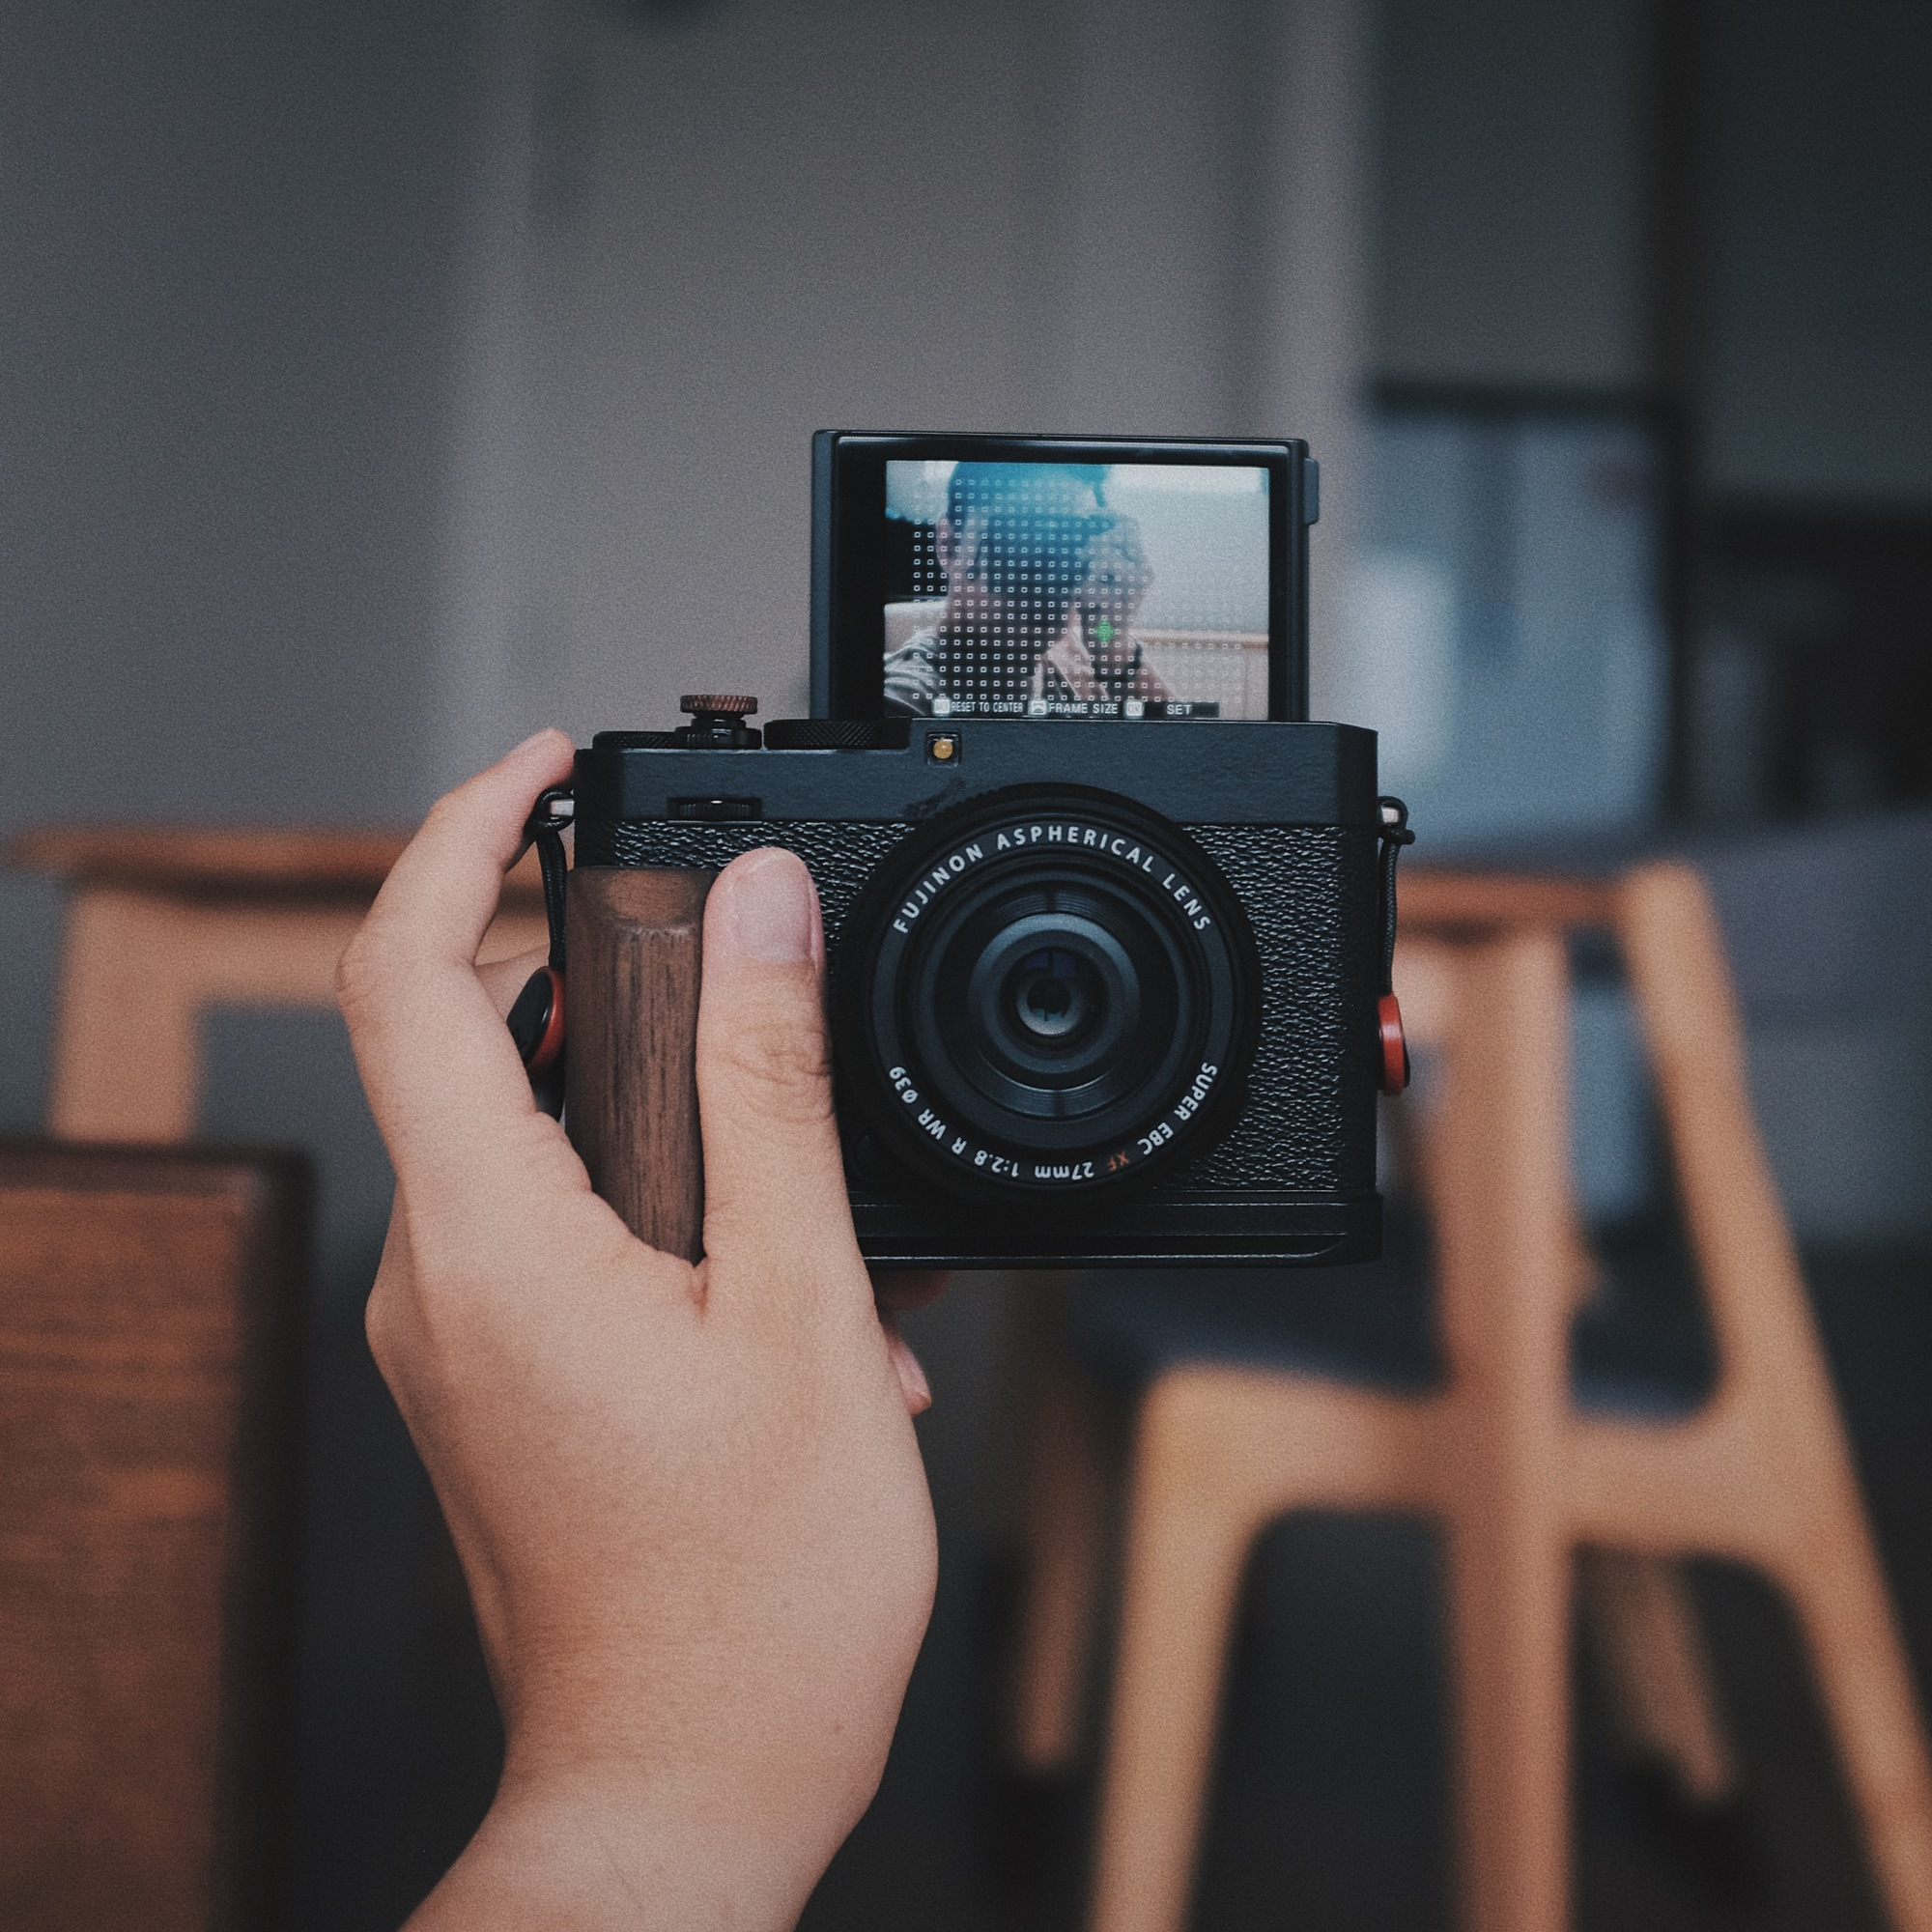
\includegraphics[width=\linewidth]{\envfinaldir/coverpic-prod.jpg}\par
            % \vskip 30pt
            \vfill

            \normalsize\rmfamily\scshape
            \copyright{} The Web Digest Project \hfill\large \envdatestr
        \end{center}
    \end{titlepage}
    % \restoregeometry
}
\newcommand{\simplehref}[1]{%
    \textcolor{blue!80!green}{\href{#1}{#1}}%
}
\renewcommand{\contentsname}{\center\Huge\sffamily\bfseries Contents\par\vskip 20pt}
\newcounter{ipartcounter}
\setcounter{ipartcounter}{0}
\newcommand{\ipart}[1]{
    % \vskip 20pt
    \clearpage
    \stepcounter{ipartcounter}
    \phantomsection
    \addcontentsline{toc}{chapter}{#1}
    % \begin{center}
    %     \Huge
    %     \sffamily\bfseries
    %     #1
    % \end{center}
    % \vskip 20pt plus 7pt
}
\newcounter{ichaptercounter}
\setcounter{ichaptercounter}{0}
\newcommand{\ichapter}[1]{
    % \vskip 20pt
    \clearpage
    \stepcounter{ichaptercounter}
    \phantomsection
    \addcontentsline{toc}{section}{\numberline{\arabic{ichaptercounter}}#1}
    \begin{center}
        \Huge
        \sffamily\bfseries
        #1
    \end{center}
    \vskip 20pt plus 7pt
}
\newcommand{\entrytitlefont}[1]{\subsection*{\raggedright\Large\sffamily\bfseries#1}}
\newcommand{\entryitemGeneric}[2]{
    % argv: title, url
    \parbox{\linewidth}{
        \entrytitlefont{#1}\par\vskip 5pt
        \footnotesize\ttfamily\mdseries
        \simplehref{#2}
    }\vskip 11pt plus 11pt minus 1pt
}
\newcommand{\entryitemGithub}[3]{
    % argv: title, url, desc
    \parbox{\linewidth}{
        \entrytitlefont{#1}\par\vskip 5pt
        \footnotesize\ttfamily\mdseries
        \simplehref{#2}\par\vskip 5pt
        \small\rmfamily\mdseries#3
    }\vskip 11pt plus 11pt minus 1pt
}
\newcommand{\entryitemAp}[3]{
    % argv: title, url, desc
    \parbox{\linewidth}{
        \entrytitlefont{#1}\par\vskip 5pt
        \footnotesize\ttfamily\mdseries
        \simplehref{#2}\par\vskip 5pt
        \small\rmfamily\mdseries#3
    }\vskip 11pt plus 11pt minus 1pt
}
\newcommand{\entryitemHackernews}[3]{
    % argv: title, hnurl, rawurl
    % \parbox{\linewidth}{
    %     \entrytitlefont{#1}\par\vskip 5pt
    %     \footnotesize\ttfamily\mdseries
    %     \simplehref{#3}\par
    %     \textcolor{black!50}{\href{#2}{#2}}
    % }\vskip 11pt plus 11pt minus 1pt
    \begin{minipage}{\linewidth}
            \entrytitlefont{#1}\par\vskip 5pt
            \footnotesize\ttfamily\mdseries
            \simplehref{#3}\par
            \textcolor{black!50}{\href{#2}{#2}}
    \end{minipage}\par\vskip 11pt plus 11pt minus 1pt
}







\begin{document}

\makeheader

\tableofcontents\clearpage




\ipart{Developers}
\ichapter{Hacker News}
\entryitemTwoLinks{Illinois bans use of artificial intelligence for mental health therapy}{https://news.ycombinator.com/item?id=44893254}{https://www.washingtonpost.com/nation/2025/08/12/illinois-ai-therapy-ban/}

\entryitemTwoLinks{Job Listing Site Highlighting H-1B Positions So Americans Can Apply}{https://news.ycombinator.com/item?id=44892321}{https://www.newsweek.com/h1b-jobs-now-american-workers-green-cards-2041404}

\entryitemTwoLinks{PYX: The next step in Python packaging}{https://news.ycombinator.com/item?id=44892209}{https://astral.sh/pyx}

\entryitemTwoLinks{US national debt reaches a record \$37T, the Treasury Department reports}{https://news.ycombinator.com/item?id=44892086}{https://apnews.com/article/treasury-debt-spending-trump-obbb-6f807c4aae78dcc96f29ff07a3c926f4}

\entryitemTwoLinks{OCaml as my primary language}{https://news.ycombinator.com/item?id=44891759}{https://xvw.lol/en/articles/why-ocaml.html}

\entryitemTwoLinks{April Fools 2014: The *Real* Test Driven Development (2014)}{https://news.ycombinator.com/item?id=44891509}{https://testing.googleblog.com/2014/04/the-real-test-driven-development.html}

\entryitemTwoLinks{A case study in bad hiring practice and how to fix it}{https://news.ycombinator.com/item?id=44890722}{https://www.tomkranz.com/blog1/a-case-study-in-bad-hiring-practice-and-how-to-fix-it}

\entryitemTwoLinks{Gartner's grift is about to unravel}{https://news.ycombinator.com/item?id=44890012}{https://dx.tips/gartner}

\entryitemTwoLinks{Nginx introduces native support for ACME protocol}{https://news.ycombinator.com/item?id=44889941}{https://blog.nginx.org/blog/native-support-for-acme-protocol}

\entryitemTwoLinks{This website is for humans}{https://news.ycombinator.com/item?id=44889627}{https://localghost.dev/blog/this-website-is-for-humans/}

\entryitemTwoLinks{New treatment eliminates bladder cancer in 82\% of patients}{https://news.ycombinator.com/item?id=44889580}{https://news.keckmedicine.org/new-treatment-eliminates-bladder-cancer-in-82-of-patients/}

\entryitemTwoLinks{Pebble Time 2* Design Reveal}{https://news.ycombinator.com/item?id=44889073}{https://ericmigi.com/blog/pebble-time-2-design-reveal/}

\entryitemTwoLinks{I'm worried it might get bad}{https://news.ycombinator.com/item?id=44888874}{https://danielmiessler.com/blog/im-worried-it-might-get-bad}

\entryitemTwoLinks{We caught companies making it harder to delete your personal data online}{https://news.ycombinator.com/item?id=44888445}{https://themarkup.org/privacy/2025/08/12/we-caught-companies-making-it-harder-to-delete-your-data}

\entryitemTwoLinks{When DEF CON partners with the U.S. Army}{https://news.ycombinator.com/item?id=44888236}{https://jackpoulson.substack.com/p/when-counterculture-and-empire-merge}

\entryitemTwoLinks{So what's the difference between plotted and printed artwork?}{https://news.ycombinator.com/item?id=44887965}{https://lostpixels.io/writings/the-difference-between-plotted-and-printed-artwork}

\entryitemTwoLinks{Pebble Time 2 Design Reveal [video]}{https://news.ycombinator.com/item?id=44887853}{https://www.youtube.com/watch?v=pcPzmDePH3E}

\entryitemTwoLinks{UK expands police facial recognition rollout with 10 new facial recognition vans}{https://news.ycombinator.com/item?id=44887373}{https://www.theregister.com/2025/08/13/uk\_expands\_police\_facial\_recognition/}

\entryitemTwoLinks{FFmpeg 8.0 adds Whisper support}{https://news.ycombinator.com/item?id=44886647}{https://code.ffmpeg.org/FFmpeg/FFmpeg/commit/13ce36fef98a3f4e6d8360c24d6b8434cbb8869b}

\entryitemTwoLinks{Nearly 1 in 3 Starlink satellites detected within the SKA-Low frequency band}{https://news.ycombinator.com/item?id=44885821}{https://astrobites.org/2025/08/12/starlink-ska-low/}\ichapter{Phoronix}
\entryitemGeneric{\hskip 0pt{}SR-IOV Will Only Be Supported On Intel Arc Pro Graphics Cards}{https://www.phoronix.com/news/Intel-SR-IOV-Only-For-Arc-Pro}

\entryitemGeneric{\hskip 0pt{}Linux Preps For New "SoC Power Slider" With Upcoming Panther Lake}{https://www.phoronix.com/news/Intel-Panther-Lake-Power-Slider}

\entryitemGeneric{\hskip 0pt{}Linux Lands Fix For Early 6.17 Regression Causing 37~43\% Performance Hit}{https://www.phoronix.com/news/Linux-6.17-Early-Regression-Fix}

\entryitemGeneric{\hskip 0pt{}Google Develops KFuzzTest For Fuzzing Internal Linux Kernel Functions}{https://www.phoronix.com/news/Linux-KFuzzTest}

\entryitemGeneric{\hskip 0pt{}Intel ISPC 1.28 Adds Optimized Support For AMD Zen 4 \& Zen 5 CPUs}{https://www.phoronix.com/news/Intel-ISPC-1.28}

\entryitemGeneric{\hskip 0pt{}Intel IDXD Accelerator Driver Cleaned Up For Some "Not So Happy Code Paths"}{https://www.phoronix.com/news/Intel-IDXD-Not-So-Happy}

\entryitemGeneric{\hskip 0pt{}Clearing The Last ReiserFS Remnants: Documentation Cleanse Of The Defunct File-System}{https://www.phoronix.com/news/ReiserFS-Documentation-Cleanse}

\entryitemGeneric{\hskip 0pt{}FFmpeg 8.0 Merges OpenAI Whisper Filter For Automatic Speech Recognition}{https://www.phoronix.com/news/FFmpeg-Lands-Whisper}

\entryitemGeneric{\hskip 0pt{}WSL2 Vulnerability Could Lead To Elevating Local Privileges}{https://www.phoronix.com/news/WSL2-CVE-2025-53788}


\ipart{Developers~~~~(zh-Hans)}
\ichapter{Solidot}
\entryitemGeneric{\hskip 0pt{}Do Kwon 对欺诈指控认罪}{https://www.solidot.org/story?sid=82032}

\entryitemGeneric{\hskip 0pt{}Perplexity 报价 345 亿美元收购 Chrome}{https://www.solidot.org/story?sid=82031}

\entryitemGeneric{\hskip 0pt{}Debian GNU/Hurd 2025 释出}{https://www.solidot.org/story?sid=82030}

\entryitemGeneric{\hskip 0pt{}亚马逊宽带卫星在轨数量突破 100 颗}{https://www.solidot.org/story?sid=82029}

\entryitemGeneric{\hskip 0pt{}有 133 亿年历史的最古老黑洞}{https://www.solidot.org/story?sid=82028}

\entryitemGeneric{\hskip 0pt{}前 NSA 局长称美国科技公司难以保持中立}{https://www.solidot.org/story?sid=82027}

\entryitemGeneric{\hskip 0pt{}柯达可能停止运营}{https://www.solidot.org/story?sid=82026}

\entryitemGeneric{\hskip 0pt{}星际译王会将 X11 剪切板数据发送到远程服务器}{https://www.solidot.org/story?sid=82025}

\entryitemGeneric{\hskip 0pt{}极端高温可能导致热带鸟类数量急剧下降}{https://www.solidot.org/story?sid=82024}

\entryitemGeneric{\hskip 0pt{}大模型的模拟推理能力只是一种脆弱的幻觉}{https://www.solidot.org/story?sid=82023}

\entryitemGeneric{\hskip 0pt{}研究发现来自人类排泄物的生物炭能解决全球化肥短缺}{https://www.solidot.org/story?sid=82022}

\entryitemGeneric{\hskip 0pt{}Reddit 将屏蔽互联网档案馆抓取其内容}{https://www.solidot.org/story?sid=82021}

\entryitemGeneric{\hskip 0pt{}掉落在居民屋顶的陨石比地球更古老}{https://www.solidot.org/story?sid=82020}

\entryitemGeneric{\hskip 0pt{}沃茨对 YouTube 的欺诈诉讼停滞不前}{https://www.solidot.org/story?sid=82019}

\entryitemGeneric{\hskip 0pt{}CEO 辞职,GitHub 不再在微软内部独立运营}{https://www.solidot.org/story?sid=82018}

\entryitemGeneric{\hskip 0pt{}高危 WinRAR 0day 正被利用}{https://www.solidot.org/story?sid=82017}

\entryitemGeneric{\hskip 0pt{}年轻血清配合骨髓细胞逆转皮肤衰老}{https://www.solidot.org/story?sid=82016}

\entryitemGeneric{\hskip 0pt{}研究发现素食者癌症风险比肉食者低 12\%}{https://www.solidot.org/story?sid=82015}

\entryitemGeneric{\hskip 0pt{}量子流体首次观测到类似梵高名画《星空》的漩涡结构}{https://www.solidot.org/story?sid=82014}

\entryitemGeneric{\hskip 0pt{}Steam 创意工坊知名模组遭遇大规模恶意 DMCA 举报}{https://www.solidot.org/story?sid=82013}\ichapter{V2EX}
\entryitemGeneric{\hskip 0pt{}[PHP] PHP 应该还是很多人用吧?}{https://www.v2ex.com/t/1152242}

\entryitemGeneric{\hskip 0pt{}[问与答] SendGrid 注册后会卡在用邮箱和用户名无法登录}{https://www.v2ex.com/t/1152241}

\entryitemGeneric{\hskip 0pt{}[电影] youku 或者芒果年卡二选一 40 元}{https://www.v2ex.com/t/1152239}

\entryitemGeneric{\hskip 0pt{}[程序员] vscode 调整缩进,差点跟 copilot 打起来}{https://www.v2ex.com/t/1152238}

\entryitemGeneric{\hskip 0pt{}[分享发现] 创业团队远程工作流程公开——《原则半远程工作手册》}{https://www.v2ex.com/t/1152237}

\entryitemGeneric{\hskip 0pt{}[投资] 如何调节自己的后悔情绪?}{https://www.v2ex.com/t/1152236}

\entryitemGeneric{\hskip 0pt{}[Solana] 关于 okex 钱包绑定 V2EX 分享}{https://www.v2ex.com/t/1152234}

\entryitemGeneric{\hskip 0pt{}[Telegram] 安卓 telegram 收取信息不及时}{https://www.v2ex.com/t/1152233}

\entryitemGeneric{\hskip 0pt{}[服务器] 阿里云服务器负载很高, iowait 占用 cpu 极高}{https://www.v2ex.com/t/1152231}

\entryitemGeneric{\hskip 0pt{}[职场话题] 工作中,对于本分以外的要求,越是举手之劳,越要学会拒绝}{https://www.v2ex.com/t/1152230}

\entryitemGeneric{\hskip 0pt{}[路由器] 求推荐公司路由器+交换机+AP}{https://www.v2ex.com/t/1152228}

\entryitemGeneric{\hskip 0pt{}[路由器] 入了小米 BE3600PRO 套装,试用发现竟然限制 p 站🤯}{https://www.v2ex.com/t/1152227}

\entryitemGeneric{\hskip 0pt{}[问与答] 很多博主认为现在年轻人(90 之后)容易被带节奏被洗脑,没独立思考能力,大家怎么看?}{https://www.v2ex.com/t/1152226}

\entryitemGeneric{\hskip 0pt{}[推广] 天翼云服务器价格}{https://www.v2ex.com/t/1152225}

\entryitemGeneric{\hskip 0pt{}[Apple] 如何选购 Macbook 电脑?更大的内存还是更先进的制程?我选择对了么?}{https://www.v2ex.com/t/1152224}

\entryitemGeneric{\hskip 0pt{}[分享发现] plancoach,下一个小猫补光灯?}{https://www.v2ex.com/t/1152223}

\entryitemGeneric{\hskip 0pt{}[加密货币] 加密货币怎么玩啊?}{https://www.v2ex.com/t/1152221}

\entryitemGeneric{\hskip 0pt{}[浏览器] Perplexity AI 要收购 Google Chrome}{https://www.v2ex.com/t/1152220}

\entryitemGeneric{\hskip 0pt{}[macOS] Mac LaunchPad 替代品推荐}{https://www.v2ex.com/t/1152219}

\entryitemGeneric{\hskip 0pt{}[程序员] 求教大佬,国内英语教材有在线的 API 获取么}{https://www.v2ex.com/t/1152218}

\entryitemGeneric{\hskip 0pt{}[程序员] 本科毕业的水平加上 ai 是否有能力做一个 C/S 架构的管理系统的软件}{https://www.v2ex.com/t/1152217}

\entryitemGeneric{\hskip 0pt{}[生活] 猜想一下,房地产税不会来,来的是房屋空置税}{https://www.v2ex.com/t/1152215}

\entryitemGeneric{\hskip 0pt{}[生活] 大学女网友 Lily 1W+的欠款近 10 年联系还上----后续}{https://www.v2ex.com/t/1152214}

\entryitemGeneric{\hskip 0pt{}[Cursor] 所以 cursor 的意思是说 9 月 15 号之前开通包年就可以在未来一年之内还能无限 auto 是吗}{https://www.v2ex.com/t/1152213}

\entryitemGeneric{\hskip 0pt{}[Android] 最近搞了一个 IP 和域名连接分析应用 IP 大院,请大家测试一下,反馈一下问题}{https://www.v2ex.com/t/1152211}

\entryitemGeneric{\hskip 0pt{}[宽带症候群] 有泉州用户吗?白名单技术机制是什么?只是 dns 的吗?}{https://www.v2ex.com/t/1152210}

\entryitemGeneric{\hskip 0pt{}[输入法] 微信输入法,没觉得多智能,无力吐槽。}{https://www.v2ex.com/t/1152207}

\entryitemGeneric{\hskip 0pt{}[奇思妙想] [灵感] 一款匹配人生轨迹的软件}{https://www.v2ex.com/t/1152206}

\entryitemGeneric{\hskip 0pt{}[程序员] 如果你觉得自身具备商业价值,你会如何展现呢?}{https://www.v2ex.com/t/1152205}

\entryitemGeneric{\hskip 0pt{}[问与答] 想攒一个可以玩 cuda 的台式机,预算 4000 内,越低越好,接受捡垃圾,大佬们有推荐的硬件搭配吗?}{https://www.v2ex.com/t/1152203}

\entryitemGeneric{\hskip 0pt{}[问与答] 有没有成熟的开源的邮件编辑器?}{https://www.v2ex.com/t/1152202}

\entryitemGeneric{\hskip 0pt{}[酷工作] [招聘] [常德] 爬虫工程师}{https://www.v2ex.com/t/1152201}

\entryitemGeneric{\hskip 0pt{}[Solana] 看到一篇出入金的帖子, 给大家分享一下, 感觉里面说的还挺中肯.}{https://www.v2ex.com/t/1152199}

\entryitemGeneric{\hskip 0pt{}[问与答] 根据你身边的案例,你预计 25 年全年的出生人口是多少}{https://www.v2ex.com/t/1152198}

\entryitemGeneric{\hskip 0pt{}[Solana] 亏块链从入门到精通}{https://www.v2ex.com/t/1152194}

\entryitemGeneric{\hskip 0pt{}[酷工作] [成都兼职] 找一名 nodejs 大佬,擅长 nestjs 更好}{https://www.v2ex.com/t/1152193}

\entryitemGeneric{\hskip 0pt{}[OpenAI] 无法在 chatgpt 关联的 onedrive 中搜索定位 PDF 文件}{https://www.v2ex.com/t/1152192}

\entryitemGeneric{\hskip 0pt{}[投资] 意外收入 1 万 5,如果丢进美股,会建议买什么?真实帖}{https://www.v2ex.com/t/1152190}

\entryitemGeneric{\hskip 0pt{}[酷工作] [上海][社招] 字节国际电商[高级/资深]前端内推大量 HC}{https://www.v2ex.com/t/1152189}

\entryitemGeneric{\hskip 0pt{}[职场话题] 想跳槽了,请各位前辈帮忙参考下 offer 是否可接}{https://www.v2ex.com/t/1152188}

\entryitemGeneric{\hskip 0pt{}[广州] 有 V 友做跨境的不。独立站的。想找个人带带。}{https://www.v2ex.com/t/1152187}

\entryitemGeneric{\hskip 0pt{}[Claude] 分享一个自己在用的 claude code hook}{https://www.v2ex.com/t/1152186}

\entryitemGeneric{\hskip 0pt{}[问与答] augment 老用户新增席位还是 30 刀?}{https://www.v2ex.com/t/1152184}

\entryitemGeneric{\hskip 0pt{}[问与答] arc 浏览器每次重启后,所有之前登录的网站都要重新登录}{https://www.v2ex.com/t/1152183}

\entryitemGeneric{\hskip 0pt{}[酷工作] 🚀 [北京/上海] MiniMax 内推 AGI 前端资深工程师}{https://www.v2ex.com/t/1152182}

\entryitemGeneric{\hskip 0pt{}[Java] 有没有比较了解 GraalVM 的,想问下适合本地开发调试吗?}{https://www.v2ex.com/t/1152181}

\entryitemGeneric{\hskip 0pt{}[求职] 小红书招聘安卓、iOS、前端工程师(正式实习均可)BASE 上海、北京}{https://www.v2ex.com/t/1152179}

\entryitemGeneric{\hskip 0pt{}[Solana] 1 美元(买断制)注册 10 位数及以上 .sol 域名倒计时。}{https://www.v2ex.com/t/1152178}

\entryitemGeneric{\hskip 0pt{}[酷工作] 小红书招聘安卓、iOS、前端工程师(正式实习均可)}{https://www.v2ex.com/t/1152176}

\entryitemGeneric{\hskip 0pt{}[奇思妙想] 有佬知道 V2EX 移动端 app 是怎么做到游客访问的吗}{https://www.v2ex.com/t/1152175}


\ipart{Generic News}







\clearpage
\leavevmode\vfill
\footnotesize

Copyright \copyright{} 2023-2025 Neruthes and other contributors.

This document is published with CC BY-NC-ND 4.0 license.

The entries listed in this newsletter may be copyrighted by their respective creators.

This newsletter is generated by the Web Digest project.

The newsletters are also delivered via Telegram channel \CJKunderline{\href{https://t.me/webdigestchannel}{https://t.me/webdigestchannel}}.\\
RSS feed is available at \CJKunderline{\href{https://webdigest.pages.dev/rss.xml}{https://webdigest.pages.dev/rss.xml}}.

This newsletter is available in PDF at
\CJKunderline{\href{https://webdigest.pages.dev/}{https://webdigest.pages.dev/}}.

The source code being used to generate this newsletter is available at\\
\CJKunderline{\href{https://github.com/neruthes/webdigest}{https://github.com/neruthes/webdigest}}.

This newsletter is also available in
\CJKunderline{\href{http://webdigest.pages.dev/readhtml/\envyear/WebDigest-20250814.html}{HTML}} and
\CJKunderline{\href{https://github.com/neruthes/webdigest/blob/master/markdown/\envyear/WebDigest-20250814.md}{Markdown}}.


\coverpic{https://unsplash.com/photos/tree-branches-reach-towards-a-clear-blue-sky-oajlEpl\_m\_w}{Fatih Berat Örer}


\end{document}
